\subsection{Energieverlust von $\alpha$-Teilchen in Materie}
Der Energieverlust von $\alpha$-Teilchen in Materie kann mit der Braggkurve, welche den Energieverlust in Abh�ngigkeit von der zur�ckgelegten Wegl�nge im Medium angibt, sowie mit der Bethe Formel, welche den Energieverlust pro Wegl�ngenelement dx in Abh�ngigkeit von der Geschwindigkeit des Teilchens angibt, beschrieben werden. Die Bethe-Formel in der relativistischen Form lautet:
\begin{align}
\label{eqn:bethe-bloch}
-\frac{dE}{dx} = \frac{4\pi n Z^2}{m_ec^2\beta^2}\left(\frac{e^2}{4\pi\varepsilon_0}\right)^2\left[\ln\left(\frac{2m_ec^2\beta^2}{I(1-\beta)^2}\right)-\beta^2\right]
\end{align}
\begin{table}[H]
\begin{tabular}{c|l}
$\beta$	&	$\frac{v}{c}$\\
$v$	&	Momentane Geschwindigkeit des Teilchens\\
$c$	&	Lichtgeschwindigkeit\\
$E$	&	Energie des Teilchens\\
$x$	&	Wegl�nge\\
$Z$	&	Kernladungszahl\\
$\varepsilon_0$	&	elektrische Feldkonstante\\
$e$	&	Elementarladung\\
$n$	&	Elektronendichte des Materials\\
$m_e$	&	Ruhemasse des Elektrons\\
$I$	&	mittleres Anregungspotential des Material\\
\end{tabular}
\end{table}
(vgl. \cite{Bethe-Formel})
Die Bethe Formel ist in Abb. \ref{fig:bethe} f�r Aluminium doppelt logarithmisch dargestellt, wobei genauere Details materialabh�ngig sind.
Die Bragg-Kurve ist in Abb. \ref{fig:braggkurve} f�r $\alpha$-Strahlung in Luft dargestellt. Das Maximum der Bragg-Kurve ist n�herungsweise gleichzusetzen mit der Reichweite des Teilchens, da der Energieverlust kurz danach auf Null absinkt.


\begin{figure}[H]
	\centering
  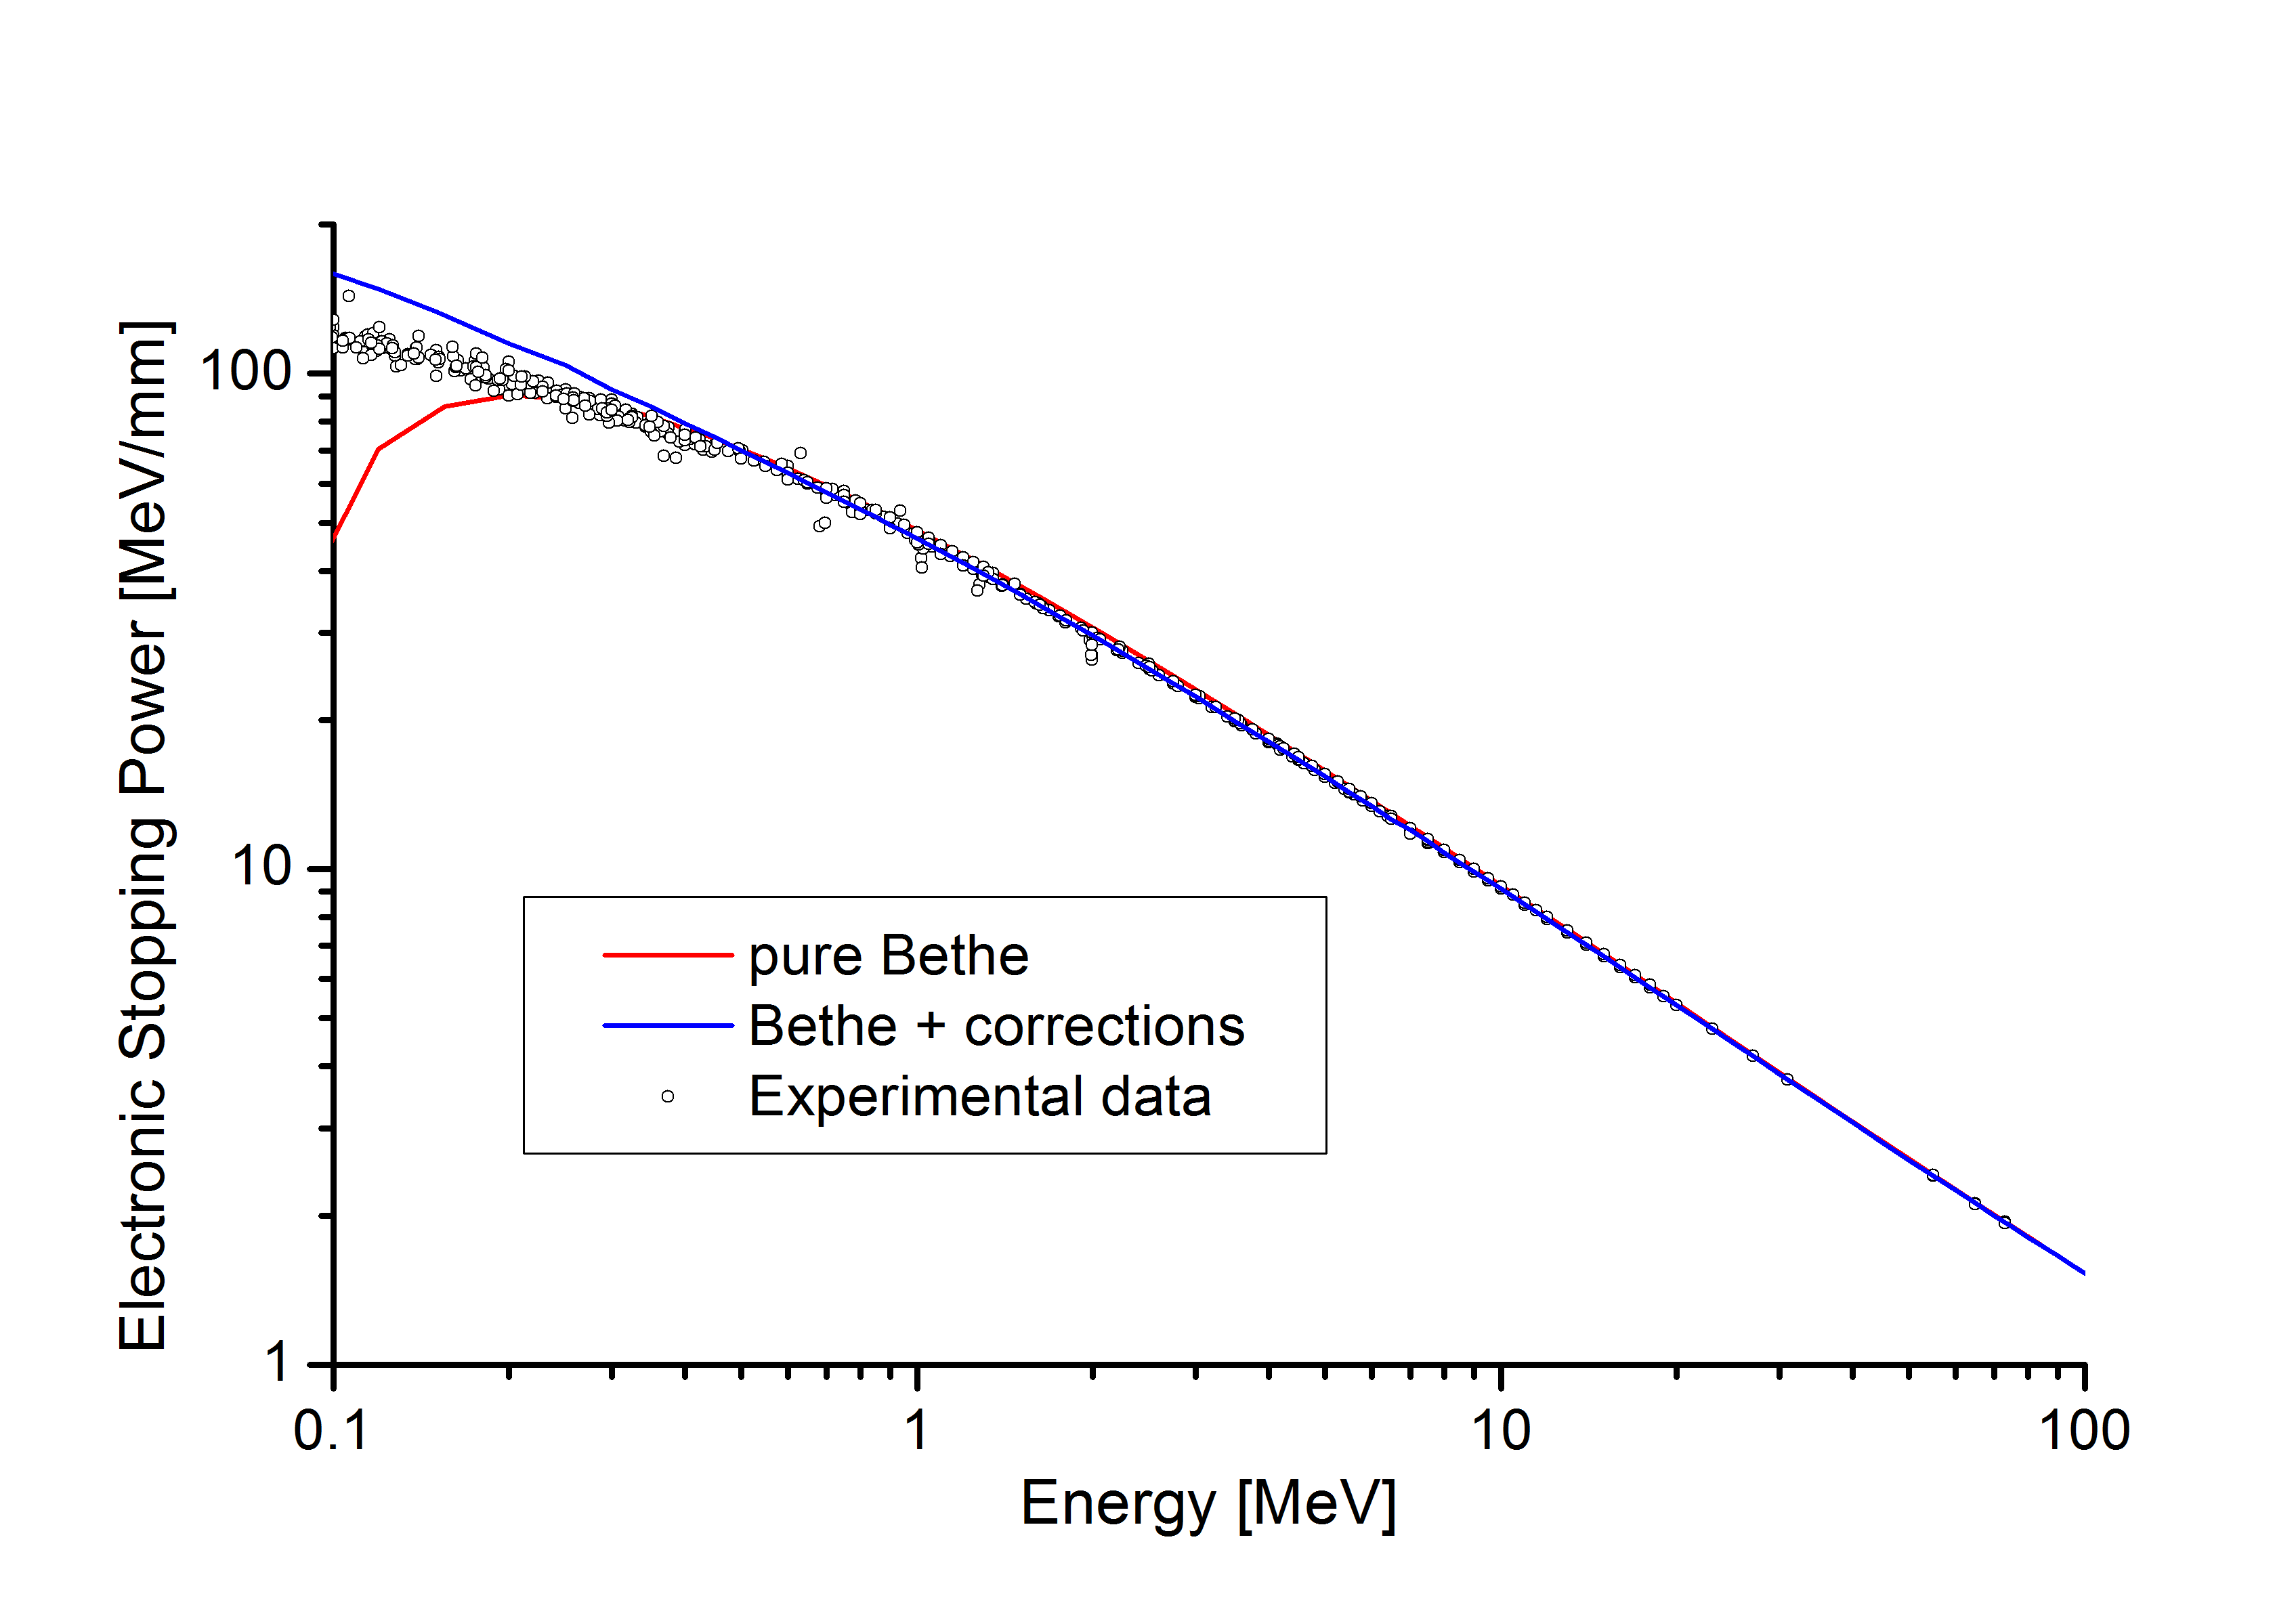
\includegraphics[scale=0.5]{Bethe.png}
	\caption{Bethe-Bloch-Kurve}
	\label{fig:bethe}
\end{figure}


\begin{figure}[H]
	\centering
  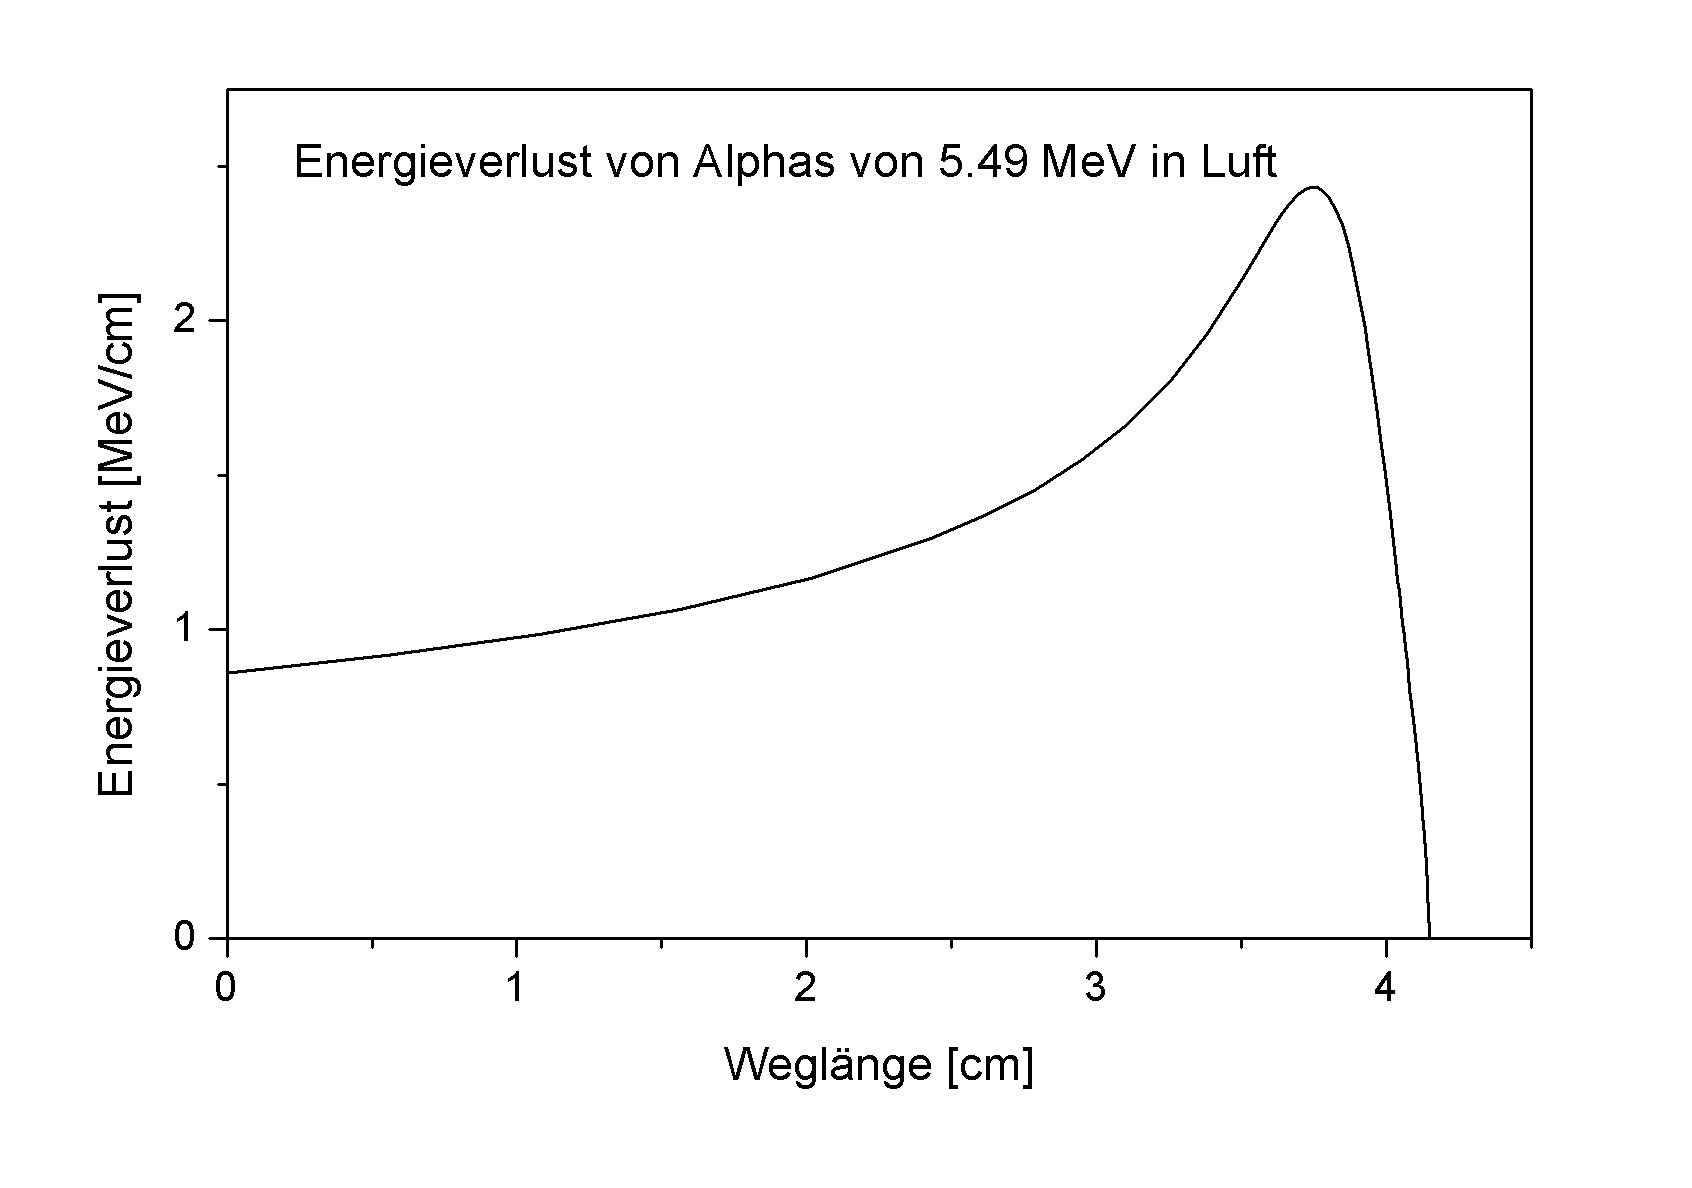
\includegraphics[scale=0.5]{Braggkurve.png}
	\caption{Braggkurve f�r $\alpha$-Strahlung in Luft}
	\label{fig:braggkurve}
\end{figure}